\subsubsection{Cálculo dos meridianos}
Os paralelos, ou caminhos ``horizontais'', são computados pelo algoritmo
descrito na subseção~\ref{paralelos}. Entretanto, o algoritmo não descreve as
transições entre linhas horizontais, como se o manipulador ``pulasse''
de um paralelo a outro, o que não pode acontecer, já que o caminho deve ser
contínuo. Dessa forma, há a necessidade de computação das curvas de transição,
os caminhos ``verticais'', ou meridianos da superfície da pá.

Ao fim da execução do cálculo de um paralelo (por exemplo, ao fim do
cálculo da curva em vermelho da figura~\ref{fig::interiso}), o
efetuador estará apontando para o último ponto com solução viável neste
paralelo, dentro das restrições de ângulo de revestimento, no lado esquerdo ou direito. A partir
deste ponto extremo (borda), o manipulador deverá ``descer'' ou ``subir'' pelo
meridiano, até encontrar outro paralelo, isto é, encontrar outra curva que
satisfaça $f(x,y,z)=g(x,y,z)$.

O método será explicado a partir de um exemplo genérico: suponha que o efetuador
do manipulador se encontra como na figura~\ref{fig::path_openrave} (borda
direita), isto é, na extremidade direita de um paralelo $c_1$. Caminhar em um
meridiano significa integrar o vetor tangente perpendicular ao encontrado por $\vec{BD} = \vec{OB} \times
\nabla{f}$, logo o caminho pelo meridiano pode ser calculado
como:
$$m_{12} = \int (\vec{OB} \times \nabla{f})\times \nabla{f} dt$$
o que irá gerar um caminho de descida pelo meridiano. Em cada passo de
integração numérica, o novo ponto $B' = B + \int_0^t (\vec{OB} \times
\nabla{f})\times \nabla{f} dt$ deve ser projetado na superfície, como em
na subseção~\ref{paralelos}, pela otimização:
$$min \left \| B-B' \right \|^2$$
$$s.t. f(B')=0$$
Além disso, em cada passo deverá ser verificado se o caminho já alcançou o
próximo paralelo $c_2$, isto é, se o ponto pertence à esfera de raio
$R_2=R_1+0.003$ (em milímetros). Observe que se o o caminho passar do próximo
paralelo, o caminho deve ser feito no sentido contrário com passo menor, isto é:
$$m_{21} = \int -(\vec{OB} \times \nabla{f})\times \nabla{f} dt$$

Na figura~\ref{fig::meridianos}, os meridianos estão representados em verde.

\begin{figure}[!ht]
	\centering
	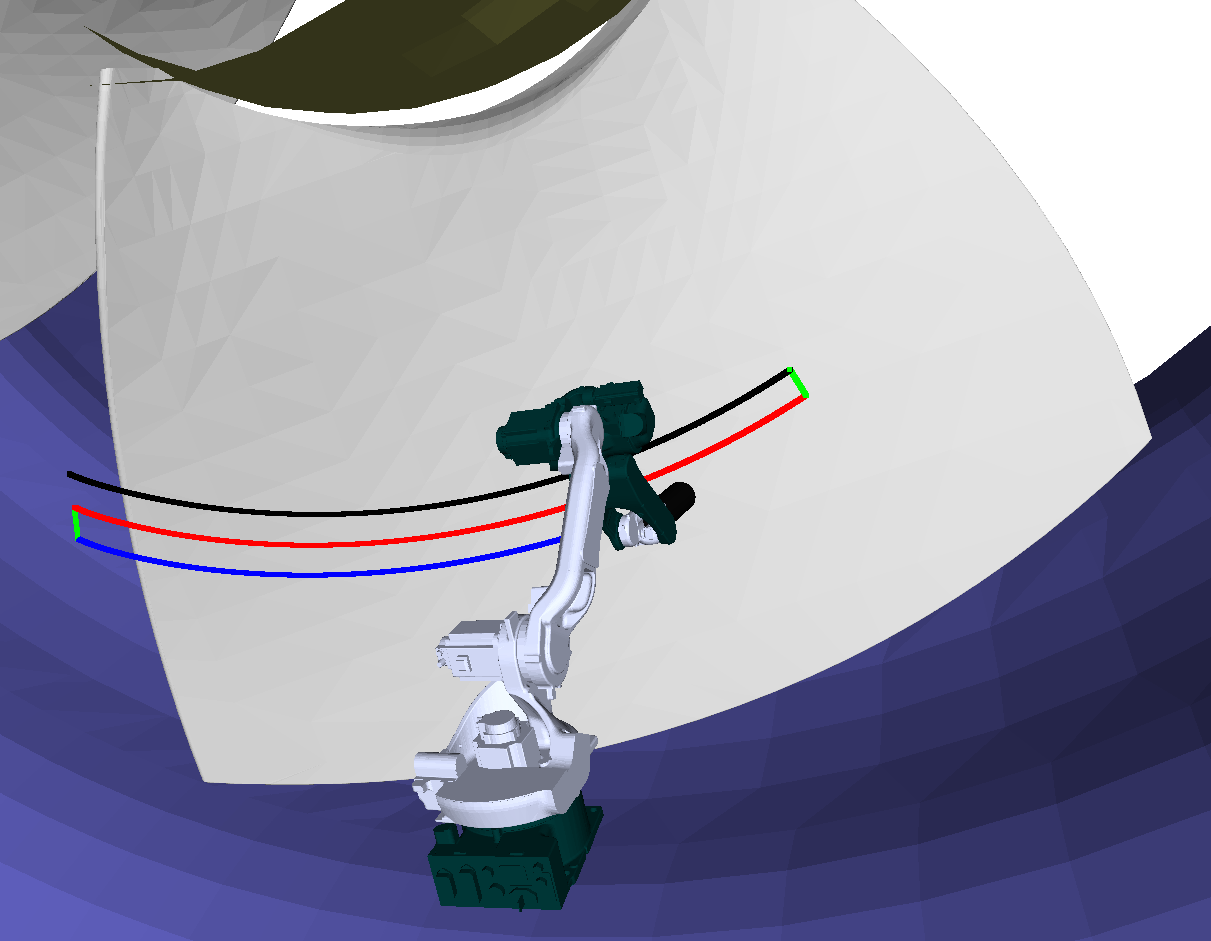
\includegraphics[width=\columnwidth]{method/figs/planejamento/meridianos.png}
	\caption{Meridianos da pá.}
	\label{fig::meridianos}
\end{figure}

\subsection{Conclusão}

No âmbito do controle e planejamento de trajetória, o método desenvolvido já se
mostrou capaz de analisar a superfície da pá, segmenta-la em regiões e definir
caminhos para serem percorridos, tanto pelo efetuador (no espaço de trabalho)
quanto pelas juntas (no espaço de juntas).

Porém, validações da precisão do resultado e análise de colisão devem ser mais
exploradas. Também devem ser julgadas pequenas modificações do método como
aplicação de minímos quadrados móveis na definição da superfície, técnica 
que possibilitaria um maior controle do erro localmente.